\documentclass[10pt,twocolumn,letterpaper]{article}
\usepackage[10pt,inchmargins]{sigmin}  %% template from Xi Wang.
\special{papersize=8.5in,11in}
\setlength{\pdfpagewidth}{8.5in}
\setlength{\pdfpageheight}{11in}
\usepackage[noheadfoot,
            left=1in,right=1in,top=1in,bottom=1in,
            columnsep=0.3in
            ]{geometry}
\usepackage[small,compact]{titlesec}
\usepackage[font={small,bf}]{caption}    % added 9/10/13
\usepackage[nolineno,noindent,norules]{lgrind}
\usepackage{tightenum}
\usepackage{float}
\usepackage{xspace}
\usepackage{times,pifont}
\usepackage{mathptmx}
\usepackage{subfig,graphics,graphicx,color}
\usepackage{multirow}
\usepackage{dblfloatfix} %% correctly orders single- and double-col figures
\usepackage{hyphenat}
\usepackage{mathrsfs}
\usepackage{subfig}
\usepackage{amssymb,amsmath,centernot}
\usepackage{lastpage}
\usepackage{flushend}
\usepackage{hhline}
\usepackage{authblk}
\newcommand{\doi}{10.1145/2797022.2797033}


%% ================= START of SOSP '13 template ================= 
 \makeatletter
 
 \def\ftype@copyrightbox{8}
 \def\@copyrightspace{
 \@float{copyrightbox}[b]
 \begin{center}
 \setlength{\unitlength}{1pc}
 \begin{picture}(20,6.8) 
 \put(0,3){\parbox{\columnwidth}{\scriptsize
 
 %*** SAMPLE. AUTHOR PUT SUPPLIED TEXT HERE ****
 
 \noindent
 \rule{6.0 cm}{0.2pt}\\
Permission to make digital or hard copies of all or part of this work for personal or classroom use is granted without fee provided that copies are not made or distributed for profit or commercial advantage and that copies bear this notice and the full citation on the first page. Copyrights for components of this work owned by others than ACM must be honored. Abstracting with credit is permitted. To copy otherwise, or republish, to post on servers or to redistribute to lists, requires prior specific permission and/or a fee. Request permissions from Permissions@acm.org.
 
 \vspace{\baselineskip}\noindent
%  Copyright is held by the Owner/Author(s).\\
 \textit{Submitted to APSys '16, August 4-5, 2016, Hong Kong, China}.\\
%  2015 ACM. ISBN 978-1-4503-3554-6/15/07\$15.00. 
%  \noindent
%  http://dx.doi.org/\doi
 }
 }
 \end{picture}
 \end{center}
 \end@float}
 
 \def\maketitle{\par
  \begingroup
    \def\thefootnote{\fnsymbol{footnote}}
    \def\@makefnmark{\hbox
        to 0pt{$^{\@thefnmark}$\hss}}
      \twocolumn[\@maketitle]
 \@thanks
  \endgroup
  \setcounter{footnote}{0}
  \let\maketitle\relax
  \let\@maketitle\relax
  \gdef\@thanks{}\gdef\@author{}\gdef\@title{}\gdef\@subtitle{}\let\thanks\relax
  \@copyrightspace}
 
 \makeatother

%% ================= END of SOSP '13 template ================= 



%\newcommand{\comment}[1]{}
\frenchspacing

%\doublespacing

%%%%%%%%%%%%%%%%%%%%%%%%%%%%
%     macro

\newcommand{\xxx}{\mbox{\textsc{Tripod}}\xspace}
\newcommand{\mytitle}[0]{\textbf {\xxx: An Efficient, Highly-available Cluster 
Management System}}
\newcommand{\mykeywords}[0]{State Machine Replication, Fault Tolerance, Stable Multithreading,
  Software Reliability}

%%%%%%%%%%%%%%%%%%%%%%%%%%%%%%%%%%%%%%%%%%%%%%%%%%%%%%%%%%%%%%%%%
% hyperref stuff

\usepackage[square,comma,numbers,sort]{natbib}
\usepackage{hypernat}
\usepackage{hyperref}

%% fill in pdf info here
\hypersetup{%
colorlinks=false,
pdfborder={0 0 0},
pdftitle={\mytitle},
pdfkeywords={\mykeywords},
bookmarksnumbered,
pdfstartview={FitH},
urlcolor=cyan,
pdfpagelabels=true,
pdfdisplaydoctitle=true,
}%

%\usepackage{breakurl}
%\usepackage[all]{hypcap}
%\renewcommand{\url}{\burl}

%%%%%%%%%%%%%%%%%%%%%%%%%%%%%%%%%%%%%%%%%%%%%%%%%%%%%%%%%%%%
% Some NICE fonts

\newfont{\BIG}{cminch}                             %--- One-inch font
\newfont{\sfbHuge}{cmssbx10 scaled\magstep5}       %-- 25pt sans serif bold
\newfont{\sfbLarger}{cmssbx10 scaled\magstep3}   %-- 12+pt sans serif boldd
\newfont{\sfblarger}{cmssbx10 scaled\magstep2}   %-- 12+pt sans serif bold
\newfont{\sfblarge}{cmssbx10 scaled\magstep1}      %-- 12pt sans serif bold
\newfont{\sfbeleven}{cmssbx10 scaled\magstephalf}  %-- 11pt sans serif bold
\newfont{\sfb}{cmssbx10}                           %-- 10pt sans serif bold
\newfont{\sfeight}{cmss8}                          %-- 8pt sans serif

%%%%%%%%%%%%%%%%%%%%%%%%
%    space tweaking

%\textwidth = 6.5 in
%\textheight = 9.0 in
%\setlength{\topmargin}{-.5in}

%\headheight = 0.0 in
%\headsep = 0.0 in
%\parskip = 0.2in
%\parindent = 0.0in

\renewcommand{\topfraction}{0.95}
\addtolength{\textfloatsep}{-0.1in}
%\addtolength{\floatsep}{0.025in}
\renewcommand\floatpagefraction{.9}
%\renewcommand\bottomfraction{.9}
\renewcommand\textfraction{.1}

\setlength{\parindent}{9pt}

% Rescue
\makeatletter
\def\v#1{{\mbox{\fontfamily{cmtt}\fontsize{\f@size}{\f@size}\selectfont #1}}}

\newcommand{\dmt}[0]{DMT\xspace}
\newcommand{\smt}[0]{StableMT\xspace}
\newcommand{\smr}[0]{SMR\xspace}
%\newcommand{\tsmr}[0]{TSMR\xspace}

\newcommand{\us}[0]{\(\mu\text{s}\)\xspace}
\newcommand{\ms}[0]{ms\xspace}
\newcommand{\paxos}[0]{\textsc{Paxos}\xspace}
\newcommand{\borg}[0]{\textsc{Borg}\xspace}
\newcommand{\calvin}[0]{\textsc{Calvin}\xspace}
\newcommand{\mesos}[0]{\textsc{Mesos}\xspace}
\newcommand{\repbox}{\mbox{\textsc{Crane}}\xspace}
\newcommand{\racepro}[0]{\textsc{RacePro}\xspace}
\newcommand{\criu}[0]{\textsc{CRIU}\xspace}
\newcommand{\tern}[0]{\textsc{Tern}\xspace}
\newcommand{\peregrine}[0]{\textsc{Peregrine}\xspace}
\newcommand{\parrot}[0]{\textsc{Parrot}\xspace}
\newcommand{\grace}[0]{Grace\xspace}
\newcommand{\coredet}[0]{\textsc{CoreDet}\xspace}
\newcommand{\kendo}[0]{Kendo\xspace}
\newcommand{\dthreads}[0]{\textsc{DThreads}\xspace}
\newcommand{\determinator}[0]{Determinator\xspace}
\newcommand{\dos}[0]{dOS\xspace}
\newcommand{\ddos}[0]{DDOS\xspace}
\newcommand{\timealgo}[0]{time bubbling\xspace}
\newcommand{\ldpreload}[0]{LD\_PRELOAD\xspace}

\newcommand{\apache}{\v{Apache}\xspace}
\newcommand{\mongoose}[0]{\v{Mongoose}\xspace}
\newcommand{\ab}{\v{ApacheBench}\xspace}
\newcommand{\clamav}{\v{ClamAV}\xspace}
\newcommand{\clamdscan}{\v{clamdscan}\xspace}
\newcommand{\drcov}{\v{drcov}\xspace}
\newcommand{\upnp}{uPnP\xspace}
\newcommand{\mediatomb}{\v{MediaTomb}\xspace}
\newcommand{\mencoder}{\v{mencoder}\xspace}
\newcommand{\mongodb}{\v{MongoDB}\xspace}
\newcommand{\ssdb}{\v{SSDB}\xspace}
\newcommand{\mysql}{\v{MySQL}\xspace}
\newcommand{\sysbench}{\v{SysBench}\xspace}
\newcommand{\zookeeper}{\v{ZooKeeper}\xspace}


\newcommand{\aget}[0]{\v{aget}\xspace}
\newcommand{\pthread}[0]{\mbox{Pthreads}\xspace}
\newcommand{\openldap}[0]{{OpenLDAP}\xspace}
\newcommand{\redis}[0]{{Redis}\xspace}
\newcommand{\bdb}[0]{{Berkeley DB}\xspace}
\newcommand{\vtune}[0]{\v{VTune}\xspace}
\newcommand{\http}[0]{\mbox{HTTP}\xspace}

% In short.
\newcommand{\eg}{{e.g.}}
\newcommand{\ie}{{i.e.}}
\newcommand{\etc}{{etc}}
\newcommand{\para}[1]{\vspace{.00in}\noindent{\bf #1}}
\newcommand{\wrt}{{w.r.t. }}
\newcommand{\cf}{{cf. }}

% Synch and network operations.
\newcommand{\mutexlock}[0]{\v{pthread\_mutex\_lock()}\xspace}
\newcommand{\connect}[0]{\v{connect()}\xspace}
\newcommand{\send}[0]{\v{send()}\xspace}
\newcommand{\close}[0]{\v{close()}\xspace}
\newcommand{\recv}[0]{\v{recv()}\xspace}
\newcommand{\select}[0]{\v{select()}\xspace}
\newcommand{\poll}[0]{\v{poll()}\xspace}
\newcommand{\epollwait}[0]{\v{epoll\_wait()}\xspace}
\newcommand{\accept}[0]{\v{accept()}\xspace}

% Parrot primitives.
\newcommand{\getturn}[0]{\v{get\_turn()}\xspace}
\newcommand{\putturn}[0]{\v{put\_turn()}\xspace}
\newcommand{\wait}[0]{\v{wait()}\xspace}
\newcommand{\signal}[0]{\v{signal()}\xspace}

% Evaluation stats.
\newcommand{\github}[0]{\url{anonymous}}
\newcommand{\ntype}[0]{three\xspace}
\newcommand{\nprog}[0]{four\xspace}
\newcommand{\overhead}[0]{1.8\%\xspace}
\newcommand{\dmtspeedup}[0]{10.5\%\xspace}
\newcommand{\proxyoverhead}[0]{1.7\%\xspace}
\newcommand{\recovertime}[0]{0.82s\xspace}
\newcommand{\mencoderspeedup}{\v{49\%}\xspace}

\newcommand{\tputoverhead}[0]{3.22\%\xspace}
\newcommand{\latencyoverhead}[0]{3.31\%\xspace}

\def\LGfsize{\footnotesize}
%\pagestyle{empty}

\begin{document}

% Hack for: Package caption Error: No float type 'copyrightbox' defined.
%\newcounter{copyrightbox}

\date{}

\title{\mytitle}

% \author[+*]{\hspace{0 mm}\fontsize{10}{10}\selectfont Heming Cui}
\author{Paper \#10}
% \author[*]{Cheng Liu}
% \author[*]{Junfeng Yang}
% \setlength{\affilsep}{1em}
% \renewcommand\AB@affilsepx{\hspace{28.0 mm}\protect\Affilfont}
%\affil[+]{Department of Computer Science}
%\renewcommand\AB@affilsepx{\\\protect\Affilfont}
%\affil[*]{Department of Computer Science\hspace{1.0mm}}
% \affil[+]{\textrm\fontsize{10}{10}\selectfont The University of Hong Kong}
% \affil[*]{\textrm Columbia University\vspace{-7.0 mm}}


\maketitle
%\thispagestyle{empty}

\begin{sloppypar}
\begin{abstract}

Nevertheless, previous approaches do not target the availability at the application 
level, but rather at the VM level, therefore service-continuity cannot be 
guaranteed in case of application failure.

This paper presents \xxx, an SMR system for KVM based virtualized machines, 
which efficiently replicates programs running in the virtual machines. 
\xxx achieves distributed consensus at the networking level of QEMU. 
Evaluation on five widely used server programs (e.g., \mysql and \redis) shows 
that \xxx is easy to use and has low overhead.

\end{abstract}
\end{sloppypar}

% \begin{sloppypar}
%% %\category{D.2.5}{Software Engineering}{Testing and Debugging}
%% \category{D.4.5}{Operating Systems}{Threads, Reliability}
%% \category{D.2.4}{Software Engineering}{Software/Program Verification}
%% \terms{Algorithms, Design, Reliability, Performance}
%% \keywords{\mykeywords}

%% \vskip 2mm
%% \noindent {\small \bf Categories and Subject Descriptors:} \vskip -.2mm
%% \noindent
%% {\footnotesize D.4.5~[{\bf Operating Systems}]: {Threads, Reliability}\\
%% D.2.4~[{\bf Software Engineering}]: {Software/Program Verification};}
%% \vskip 1mm
%% \noindent {\small \bf General Terms:} \vskip -.2mm
%% \noindent
%% {\footnotesize Algorithms, Design, Reliability, Performance}
%% \vskip 1mm
%% \noindent {\small \bf Keywords:} \vskip -.2mm
%% \noindent
%% {\footnotesize \mykeywords}

% \vskip 2mm
% \noindent {\small \bf Categories and Subject Descriptors:}
% {\small D.4.5~[{\bf Operating Systems}]: {Threads, Reliability};
%   D.2.4~[{\bf Software Engineering}]: {Software/Program Verification};}
% \vskip .1mm
% \noindent {\small \bf General Terms:} {\small Algorithms, Design,
%   Reliability, Performance}
% \vskip .1mm
% \noindent {\small \bf Keywords:} {\small \mykeywords}
% 
% \end{sloppypar}

%%%%%%%%%%%%%%%%%%%%%%%%%%%%%%%%%%%
% Add page number.
\setcounter{page}{1}
\pagenumbering{arabic}

\thispagestyle{plain}
\pagestyle{plain}
\setlength{\footskip}{20pt}
%%%%%%%%%%%%%%%%%%%%%%%%%%%%%%%%%%%

\begin{sloppypar}

\section{Introduction} \label{sec:intro}

% P1: virtualization is good
By allowing multiple servers to be consolidated on a small number of physical hosts 
and simplifying provisioning, virtualization is widely used in computing environments 
of various kinds and scales.

% P2: However, previous approaches still fail to efficiently and reliably provide fault-tolerance in virtualized environment
% checkpoint-recovery based replication suffers from two problems
% 1. performance degradation due to the large amount of state that needs to be synchronized between the primary and the backup machines
% 2. significant VM downtimes
% 3. network delay
Nevertheless, server consolidation exacerbates the consequence of unexpected host failures. 
When VMs are consolidated, failure of a single host may bring down mutiple VMs on the host 
and all applications running thereon, resulting in an unacceptable aggregate loss. 
To accommdote virtual machines with high availability, various approaches have been 
proposed to replicate VMs between hosts continuously throughout VM's execution, but 
they are still unable to ensure fault-tolerance in virtualized environments efficiently 
and reliably. One typical technique is checkpoint-recovery based replication of virtual 
machines. It captures the entire execution state of the running VM at relatively 
high frequency so that changes can be reflected to the backup machine nearly instantly. 
One disadvantage of the checkpoint-recovery based replication is the amount of data that 
needs to be copied from the primary to the backup, which can, in some cases, seriously 
affect the performance. Apart from that, VM downtimes incurred by the checkpoint mechanism 
can be significant.

% P3: derterministic replay is the other approach which can address some of the drawbacks of checkpoint-recovery based replication
% single point of failure
% slow for multi-processor

% To answer Heming's question: old leader and new leader get to an inconsistent state
% After recovery, the old leader should be started in the state as the new leader before participating

% 6.824 2016 mit
% What if the network between primary/backup fails?
%  -Primary is still running
%  -Backup becomes a new primary
%  -Two primaries at the same time!
% one can avoid split brain using a single "master"
% master computer decides whether replica A or replica B is the primary
%   there's just one master, so it never disagrees with itself
% clients talk to the master
% this is probably what VMware FT does (atomic test-and-set in shared disk)
% but what if the master fails?
%   it's a "single point of failure" -- not so good
% VMware FT shared disk atomic test-and-set was (apparently) not replicated

% In the non-shared-disk configuration, there may be no shared storage to use for dealing with a split-brain situation.
% In this case, the system could use some other external tiebreaker, such as a third-party server that both servers can talk to.
% If the servers are part of a cluster, the system could alternatively use a majority algorithm based on cluster membership.

On the other hand, derterministic replay is an attractive technique which can address the 
aforementioned drawbacks of checkpoint-recovery based replication: primary and backup execute 
the same sequence of instructions, with non-deterministic events injected exactly at the same 
point into both replicas. However, in the existing works, in order to avoid split brain, 
derterministic replay has to suffer from "single point of failure".

Fortunately, \paxos, a majorty vote algorithm, can be used to prevent the split-brain scenarios 
across the cluster. Moreover,  \paxos provides another great benefit: it ensures the same sequence 
of input requests for replicas. But \paxos is notoriously slow because each decision takes at least 
three message delays between when a replica proposes a command and when some replica learns which 
command has been chosen.

Luckily, Remote Direct Memory Access (RDMA)-capable networks have dropped in price and made 
substantial inroads into datacenters. It allows one computer to directly access the memory of 
a remote computer without involving the operating system at any host. This enables zero-copy 
transfers, reducing latency and CPU overhead.

The remainder of the paper is organized as follows.

\section{Background} \label{sec:background}

% TBD.

\subsection{\paxos}\label{sec:paxos}
% \paxos background. Keys:
% Leader, backup.
% Persistent storage. 
% Network round trips in normal case. Latency.
An SMR system runs the same program and its data on a set of machines 
(replicas), and it uses a distributed consensus protocol (typically, 
\paxos~\cite{paxos:complex,paxos,paxos:simple,paxos:live,paxos:fast,
paxos:practical}) to coordinates inputs across replicas. For efficiency, in 
normal case, \paxos often lets one replica work as the leader which invokes 
consensus requests, and the other replicas work as backups to agree on or 
reject 
these requests. If the leader fails, \paxos elects a new leader from the 
backups.

Two main reliability features must be enforced in a standard \paxos protocol. 
The first one is durability. When a new input comes, the \paxos leader writes 
this input in local stable storage. The leader then starts a new consensus 
round, which invokes a consensus request on ``processing this input" to the 
other backups. A backup also writes the received consensus request in local 
storage if it agrees on this request. Durability ensures that even if the 
leader or backups fail and restart, they can still retrieve the requests from 
local stable storage and re-execute them.

The second feature is safety. As long as a quorum (typically, majority) of 
replicas agree on this input (\ie, this input is \emph{committed}), \paxos 
guarantees that all replicas consistently agree to process this input. If a 
replica sees that an input consensus has been reached, this consensus must have 
really been reached by at least a majority of replicas. Safety ensures that if 
a consensus has not really been reached, no replica will ``think" that this 
consensus has been reached.

Durability and safety make replicas consistently agree on each input and 
tolerate various faults, including machine failures and network errors. As 
consensus rounds move on, \paxos consistently enforces the same sequence of 
inputs across replicas. It also enforces same execution states across replicas 
without divergence if a program behaves as a deterministic state machine (\ie, 
always produces the same output on the same input).

% Normal case, round trip.
Network latency of consensus messages is one key problem to make general server 
programs adopt SMR. For instance, in an efficient, practical 
\paxos implementation~\cite{paxos:practical}, each input in normal case takes 
one consensus round-trip between every two replicas (one request from the 
leader and one reply from a backup).

\subsection{RDMA} \label{sec:rdma}

RDMA architecture such as Infiniband~\cite{infiniband} or RoCE~\cite{roce} 
recently becomes commonplace in datacenters due to its extreme low latency, 
high throughput, and its decreasing prices. 

RDMA provides three types of communication primitives, from slowest to 
fastest: IPoIB (IP over Infiniband), message verbs, and one-sided read/write 
operations. A one-sided RDMA read/write operation can directly write from one 
replica's memory to a remote replica's memory, completely bypassing OS kernel 
and CPU of the remote replica. For brevity, the rest of this paper denotes a 
one-sided RDMA write operation as a ``WRITE".


% \subsection{State Machine Replication (\smr)} \label{sec:smr}

% State machine replication (\smr) is a powerful fault-tolerance
% concept~\cite{paxos:practical}.  It models a program as a deterministic state 
% machine, where states are important program data and the transitions are 
% deterministic executions of program code under input requests.  \smr runs 
% replicas of this state machine on multiple nodes, tolerating many possible node 
% and network failures.  To keep the replicas consistent, it invokes a
% distributed consensus protocol (typically \paxos~\cite{paxos, paxos:simple, 
% paxos:practical}) to ensure that a quorum (typically majority) of the replicas 
% agree on the input request sequence; under the deterministic execution 
% assumption, this quorum of replicas must reach the same exact state.  \smr is 
% proven safe in theory, and provides high availability in practice.
% 
% To support general server programs transparently, \repbox leverages \repbox's 
% \paxos consensus protocol, which takes the POSIX socket API as
% consensus interface. This \paxos protocol enforces two kinds of 
% orders for socket operations. First, for requests coming from the clients, 
% such as \connect and \send requests, this protocol enforces that all nodes see 
% the same totally ordered sequence of these requests using the \paxos and socket 
% API interposition components.  (this protocol does not need to order the 
% blocking socket operations in the clients because we mainly focus on analyses 
% for server applications.) Second, for server applications' blocking operations, 
% this \paxos protocol schedules them according to the matching operations from 
% the clients (\eg, a \send from a client matches a \recv from the server within 
% the same socket connection). This protocol does not schedule non-blocking 
% operations in servers (\eg, \send to clients) because it focuses on replicating 
% the server's execution states.
% 
% % For practicality, \repbox's \paxos implementation takes a well-known 
% % engineering approach~\cite{paxos:practical}: only the primary invokes consensus 
% % request during normal operations, and an leader election is invoked when 
% % exceptions such as network partitions occur.
% 
% 
% Figure~\ref{fig:repbox} shows an instance of \repbox running on 
% each node, and the \paxos consensus component is the gateway of this instance.  This 
% component accepts socket requests from the clients and invoke a \paxos 
% consensus instance with the other replicas on this operation. Once a consensus 
% is reached, this component forwards the operation to the \dmt component. This 
% component is also the only \repbox component that communicates among different 
% \repbox instances. 
% 
% In this paper, \xxx skips the fault-tolerance nature of \repbox, but leverages it 
% to construct multiple equivalent executions for analysis tools.
% 
% \subsection{Deterministic Multithreading (\dmt)} \label{sec:dmt}
% 
% \dmt~\cite{dpj:oopsla09, 
% dmp:asplos09, kendo:asplos09, coredet:asplos10, dos:osdi10, ddos:asplos13, 
% ics:oopsla13} is an advanced threading technique that enforces the same 
% schedule 
% on the same inputs.  This technique typically maintains a \emph{logical
%   time}\footnote{Though related, the logical time in \dmt is not to be
%   confused with the logical time in distributed
%   systems~\cite{lamportclock}.} that advances deterministically based on
% the code run.  It allows a thread to synchronize only at deterministic
% logical times.  By induction, it makes an entire multithreaded execution
% deterministic.  The overhead of \dmt is typically moderate: one recent
% \dmt system, \parrot~\cite{parrot:sosp13}, incurs an average of 12.7\%
% overhead on a wide range of 108 popular multithreaded programs on 24-core
% machines.
% 
% The \dmt component in Figure~\ref{fig:repbox} runs within the same process as a server replica, and
% enforces the same logical clocks for inter-thread communication
% operations. \repbox leverages the \parrot~\cite{parrot:sosp13} \dmt runtime
% system because it is fast (\ie, 12.7\% overhead for a wide range of 108 popular 
% multithreaded programs) and transparent to the application.
% 
% 
% Specifically, \parrot uses a runtime technique called \ldpreload to dynamically 
% intercept \pthread synchronizations (\eg, \mutexlock) issued by an executable 
% and enforces a well-define, round-robin schedule on these synchronization 
% operations for all threads, practically eliminating nondeterminism in thread
% synchronizations. Although \parrot is not designed to resolve data races
% deterministically, deploying a race detector in one replica can overcome this 
% limitation (\S\ref{sec:discuss}).  \repbox augments the \dmt component to schedule 
% the return points of blocking socket operations in server replicas, too, to 
% ensure that requests are admitted exactly at the same logical time across 
% replicas.



% Our model. Multiple writer multiple reader.
\section{\xxx Overview} \label{sec:overview}

This section first introduces \xxx's architecture design (\S\ref{sec:arch}), 
its workflow on scheduling tasks with replication (\S\ref{sec:workflow}), and 
its trade-off on reliability versus resource consumption (\S\ref{sec:discuss}).

% TBD. 

\subsection{Architecture} \label{sec:arch}

\xxx's deployment model is similar to a typical cluster management system's 
(\eg,~\cite{borg:eurosys15,mesos:nsdi11}). \xxx has a replicas of three to five 
controllers, with each connects with the others using high-speed RDMA network. A 
controller is elected by \paxos a the leading controller, which propose 
consensus requests to execute tasks. The other controllers are standby 
controllers which agree on or reject consensus requests. A number of slave 
machines act as computational resources that hold applications' running tasks. 
Controllers and slaves connect with either RDMA or TCP/IP. Application 
schedulers submit tasks to the leader controller.

\begin{figure}[t]
\vspace{.20in}
\centering
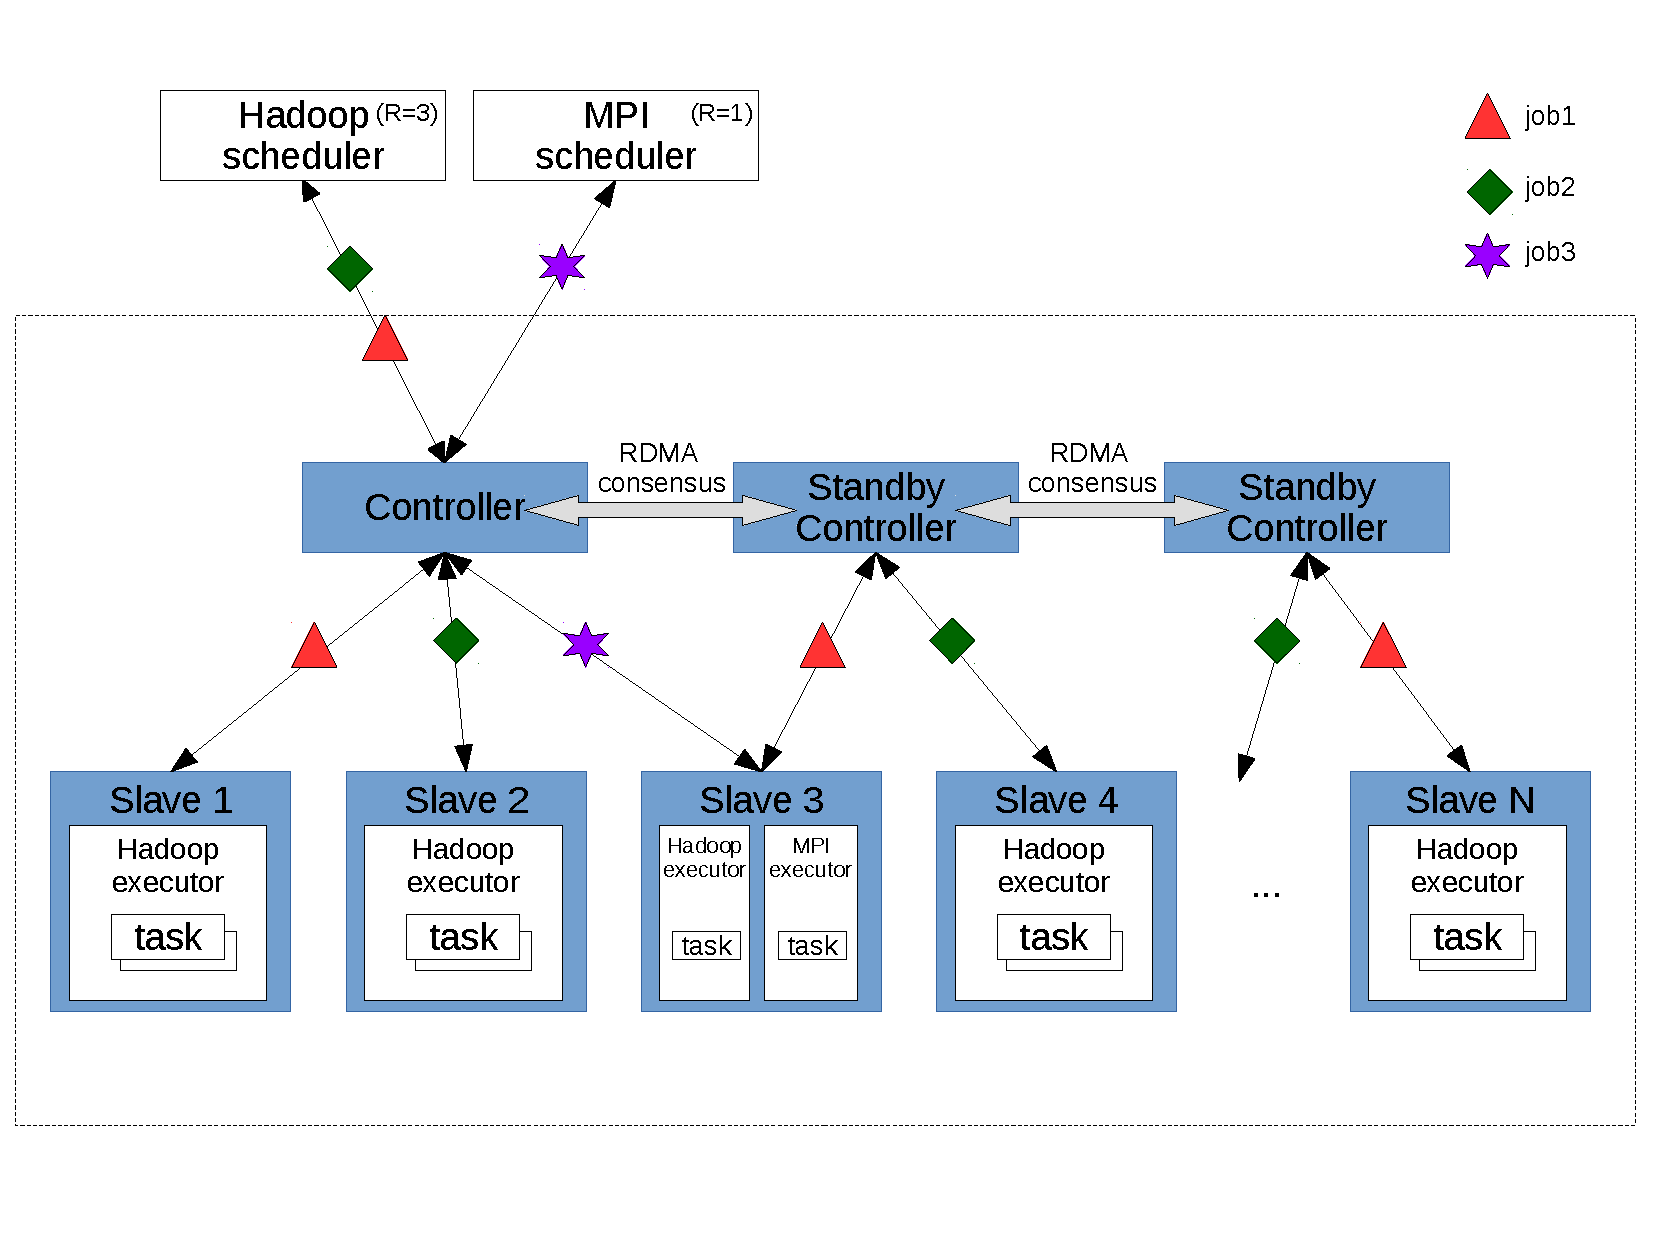
\includegraphics[width=.47\textwidth]{figures/arch}
\vspace{.06in}
\caption{{\em The \xxx Architecture.} Key components are shaded (and 
in blue).} \label{fig:arch}
\vspace{-.05in}
\end{figure}

Figure~\ref{fig:arch} depicts \xxx's architecture, and its key components are 
shaded (and in blue). To illustrate how \xxx works in an application 
perspective, this figure shows two applications, Hadoop and MPI. Each 
application has a \emph{replica strength} (R) to denote the level of 
fault-tolerance it demands. This value is either 1 or equals the number of 
replicas of controllers in \xxx. By default, each application has \v{R=1}, 
which means that this application does not need replication. For such a default 
setting, \xxx runs the task as is without replication, like a typical cluster 
management system (\eg, Mesos).

In this figure, Hadoop's R is 3, which means that it wants to replica each of 
its task in three replicas for high-availability. Suppose Hadoop submits two 
tasks to the leader controller, each has different shapes (triangle or 
hexagon). The leader controller thens invokes a consensus on each task across 
controllers. Once a consensus is reached, each controller assigns the same task 
on different slave machines.

The leader controller returns its task computation result to the Hadoop 
scheduler unless a tail-tolerance mechanism is triggered 
(\S\ref{sec:workflow}). standby controllers ignore the results of their tasks 
unless this mechanism is triggered.



\subsection{Workflow on Scheduling Tasks} \label{sec:workflow}

\begin{figure}[t]
\vspace{.20in}
\centering
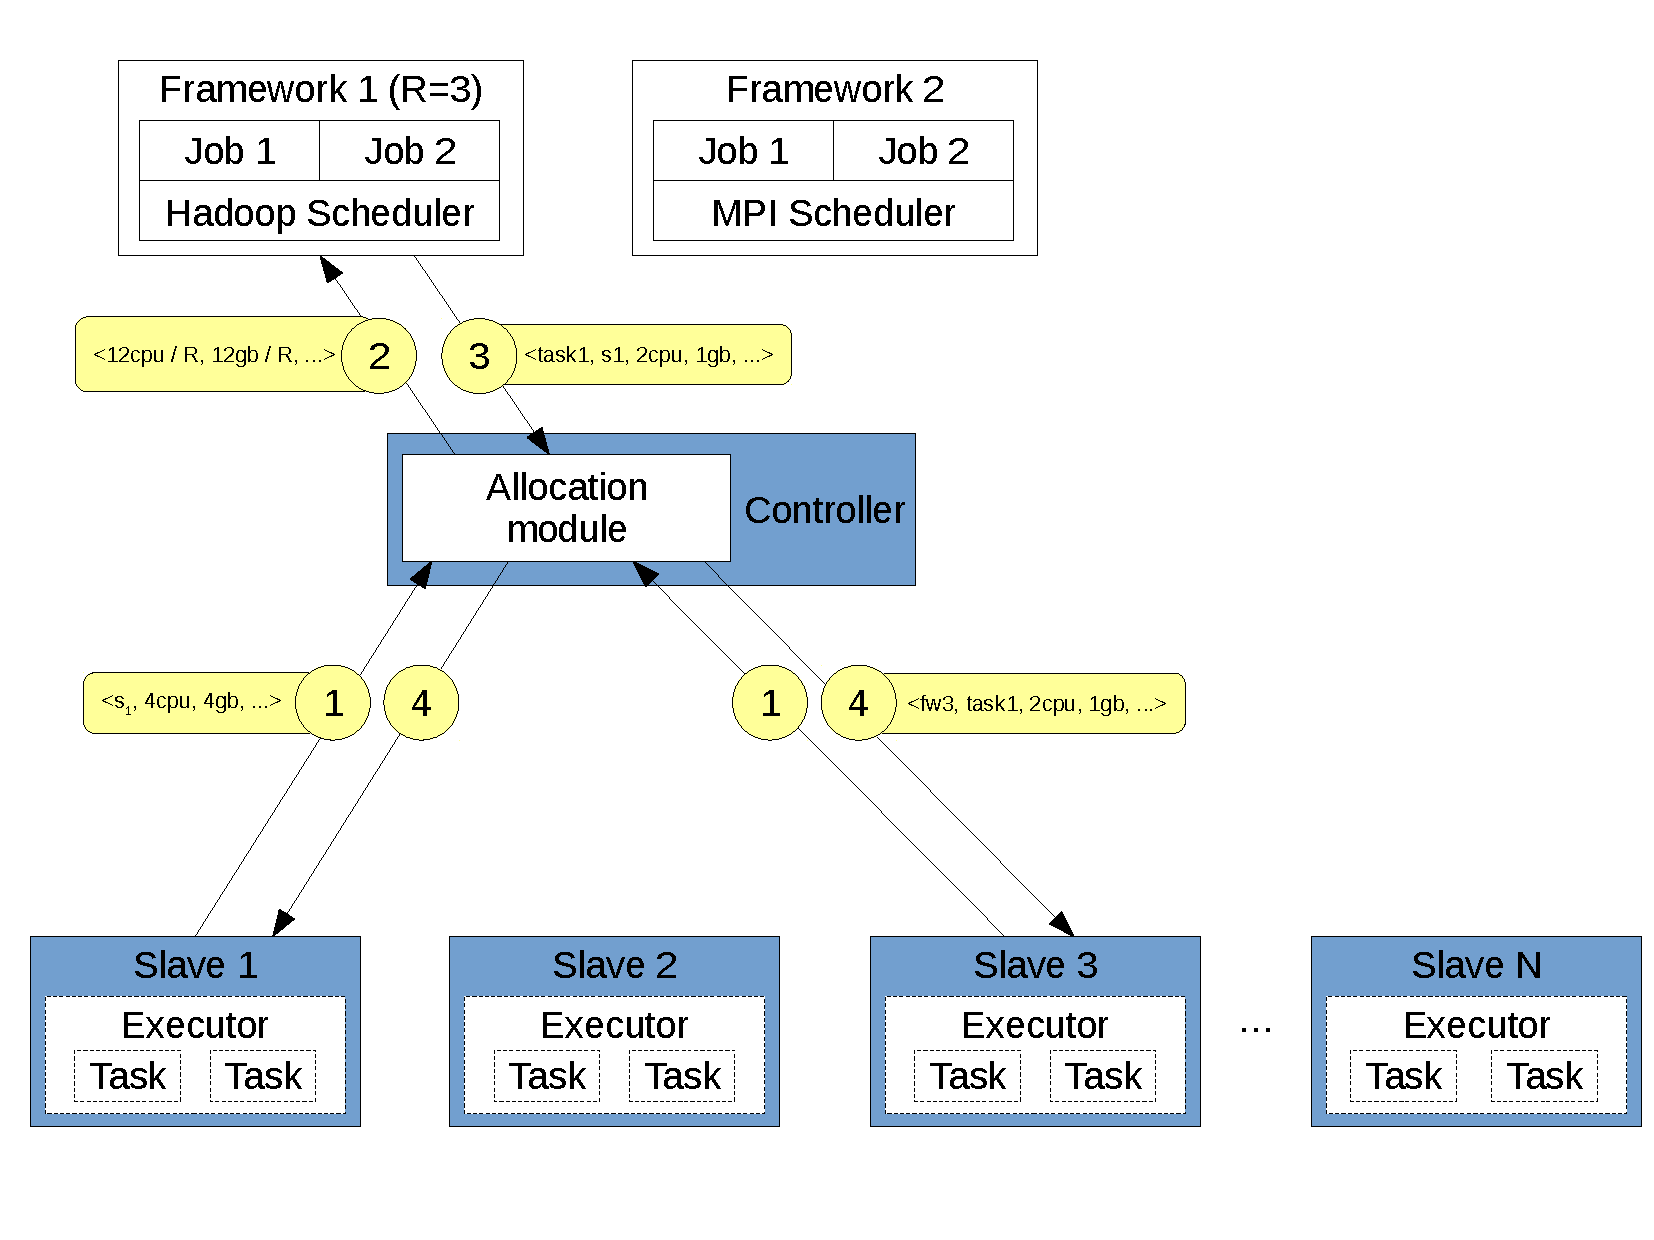
\includegraphics[width=.47\textwidth]{figures/flow}
\vspace{.06in}
\caption{{\em The \xxx Workflow on Scheduling Tasks.}} \label{fig:workflow}
\vspace{-.05in}
\end{figure}

Figure~\ref{fig:workflow} shows \xxx's workflow on scheduling tasks with four 
steps. This workflow is similar to that in Mesos except the second and fourth 
steps. These two steps \xxx abstract away the replication logic in its resource 
offers and allocations from the application. An application runs as if \xxx does 
not replicate any of its tasks, and \xxx handles all the replication logic.

In the first step, slave machines periodically report their available computing 
resources (\eg, CPU cores and memory) to the leader controller. In the second 
step, instead of reporting available resources, \xxx divides the amount of 
resources by each application's \v{R} value and then reports to the 
application. This is to reserve enough resources for \xxx to replicate the same 
task with \v{R} copies.

In the third step, an application scheduler submits tasks to the leader 
controller. The leader controller then invokes a consensus on this task by 
carrying the resource offer made to the application.

Once a majority of controllers agrees on executing this task, each controller 
does the fourth task. It schedules this task on an available slave machine 
according to the resource offer. To avoid controllers putting the same task on 
the same slave machine, each controller maintains a disjoint bit-mask of slave 
machines; it only schedules this task on machines belongs to its bit-mask if 
this machine has available resource to hold this task.

% More discussions, frangmentation, 4+1+1, not available to hole 3*2. 
% But critical applications, resource is often not a bottleneck compared to 
% response time and availability.

\subsection{Discussion} \label{sec:discuss}

The main goal of \xxx is to provide high-availability to critical applications 
running in clusters. On one hand, clusters are included more and more computing 
resources (\eg, machines), where failures of these resources and applications 
are already commonplace~\cite{facebook:outage}. On the other hand, 
high requirements on response times and availability become more and more 
important to critical applications. For instance, Both NYSE and Nasdaq have 
experienced outage of their whole site~\cite{nyse:halt} or specific IPO 
events~\cite{facebook:ipo:delay} due to minor machine errors.  Even social 
networking applications like Facebook has strong fault-tolerance requirements, 
because minor machine failures have turned down the whole Facebook site for 
several times in the last few years~\cite{facebook:outage}, costing huge 
money lost. 

Therefore, \xxx's design favors more on availability and performance 
(low consensus latency). It's design tends to use \v{R} times of resources 
compared to traditional applications. We argue that this extra resource 
utilizations are acceptable for critical applications, because if they have high 
demand on availability and response times, they can often tolerate costs on 
computing resources (\eg, trading and medical platforms).


\section{Tail-tolerance Design} \label{sec:tail}

\xxx's tail tolerance design is based on its \paxos consensus protocol. This 
design consists of three steps. First, for each job request, both the leader 
controller and standby controllers schedule the same job and receive output of 
this job. When each standby controller receives a job output, it 
uses RDMA WRITEs to write back their job outputs to the leader master's local 
memory.

Second, the leader master also waits for its own job output and frequently 
polls from the other replicas' outputs for this job. Third, if the leader finds 
that standby masters have already written back an output for a job, it sends 
back the output to the application scheduler and ignores its own job output. 
This guarantees that application schedulers receive job outputs without being 
affected by stragglers in minor replicated jobs.

Although \xxx is not the first work that presents a replication approach to 
address the straggler problem (\eg, Dolly~\cite{dolly:nsdi13}), \xxx's 
tail-tolerance design has two practical benefits. First, \xxx's design is 
simple and general to applications, because it is built on top of its \paxos 
replication architecture without extra replication logic. Second, the standby 
masters' output write-back are fast through RDMA writes. 
% \newpage
\section{Evaluation} \label{sec:eval}

% We evaluated an anti-virus scanning server that a b c d e f.

\begin{table}[b]
\footnotesize
\centering
\vspace{-.05in}
\begin{tabular}{lrrr}
{\bf Approach} & {\bf Resp time (s)} & {\bf Overhead (\%)} \\
\hline\\[-2.3ex]
Native execution                       & 1.14  &        \\
\xxx framework only                       & 3.03   & 0     \\
\xxx with Helgrind                                   & 20.96 & 0     \\
\xxx with Helgrind and XX                       & 23.76 & 0       \\
Helgrind only                       & 23.76 & 0       \\
\end{tabular}
\vspace{-.05in}
\caption{{\em Percentage of inserted time bubbles among all consensus 
requests.}} 
\label{tab:bubble-percentage}
\end{table}

We evaluated \xxx on \clamav, an anti-virus scanning server that scans files 
parallely and deletes malicious ones. Our evaluation was done on a set of three 
Linux 3.2.14 machines within a 1Gbps bandwidth LAN, and each machine has 2.80 
GHz dual-socket hex-core Intel Xeon with 24 hyper-threading cores and 64GB 
memory. we used \clamav's own client utility \v{clamdscan} to request the server 
to parallely scan \clamav's own source code and installation directories. we 
measured each workload's response time because it has direct impact on users.


\section{Related Work} \label{sec:related}

\para{Cluster Management System.} Cluster management 
systems~\cite{borg:eurosys15,mesos:nsdi11,tupperware,yarn:socc13,
autopilot:sosp07,quincy:sosp09,apollo:osdi14,fuxi:vldb14} are widespread 
because they can transparently support many diverse applications (\eg, 
Hadoop~\cite{hadoop}, Dryad~\cite{dryad}, and key-value stores~\cite{redis}). 
These existing systems mainly focus on high availability for themselves by 
replicating important components (\eg, controllers) within these systems, or 
focus on fault-recovery of applications~\cite{fuxi:vldb14}. To the best of our 
knowledge, no existing system provides efficient and general high-availability 
service to applications. Although \xxx's current design leverages an existing 
system Mesos~\cite{mesos:nsdi11}, its general \paxos protocol design can also 
be integrated in other systems.

\para{State machine replication (SMR).}  SMR is a powerful, but 
complex fault-tolerance technique. The literature has developeed a rich set of
\paxos 
algorithms~\cite{paxos:practical,paxos,paxos:simple,paxos:complex,epaxos:sosp13}
and implementations~\cite{paxos:live,paxos:practical,chubby:osdi}. \paxos is 
notoriously difficult to be fast and scalable~\cite{ellis:thesis}. To improve 
speed and scalability, various advanced replication models have been 
developed~\cite{epaxos:sosp13,mencius:osdi08,scatter:sosp11,manos:hotdep10}. 
Since consensus protocols play a core role in 
datacenters~\cite{matei:hotcloud11, mesos:nsdi11, datacenter:os} and 
distributed 
systems~\cite{spanner:osdi12,mencius:osdi08}, a variety of study have been 
conducted to improve different aspects of consensus protocols, including 
performance~\cite{epaxos:sosp13,paxos:fast,dare:hpdc15}, 
understandability~\cite{raft:usenix14,paxos}, and verifiable reliability 
rules~\cite{modist:nsdi09,demeter:sosp11}. Although \xxx tightly integrates 
RDMA features in \paxos, its implementation mostly complies with a popular, 
practical approach~\cite{paxos:practical} for reliability. Other \paxos 
approaches can also be leveraged in \xxx.

\para{RDMA techniques.} RDMA techniques have been implemented in various 
architectures, including Infiniband~\cite{infiniband}, RoCE~\cite{roce}, and 
iWRAP~\cite{iwrap}. RDMA have been leveraged in many systems to improve 
application-specific latency and throughput, including high performance 
computing~\cite{openmpi}, key-value 
stores~\cite{pilaf:usenix14,herd:sigcomm14,farm:nsdi14,memcached:rdma}, 
transactional processing systems~\cite{drtm:sosp15,farm:sosp15}, and file 
systems~\cite{gibson:nfs}. These systems are largely complementary to \xxx.
% It 
% will be interesting to investigate whether \xxx can improve the availability 
% for 
% both the client and server for some of these advanced systems within a 
% datacenter, and we leave it for future work.
\section{Conclusion} \label{sec:conclusion}

We have presented \xxx, an efficient, transparent dynamic program analysis 
framework. It leverages \smr and \dmt to consturct multiple equavalent 
executions in replicas, so that actual executions and analyses can be fully 
decoupled. Evaluation shows that \xxx can transparently run analyses on 
replicas with reasonable overhead. Furthermore, analyses and \xxx can be 
mutually beneficial. \xxx has the potential to promote the deployments of 
powerful analyses in applications' production runs.
\end{sloppypar}

% uncomment to tweak with bib spacing
%\setlength\bibsep{2.25pt}
{
%\small
 \bibliographystyle{abbrv}
 \bibliography{bib/biblio}
}

\end{document}
